\documentclass[12pt]{article}
\usepackage{palatino}
\usepackage{fullpage}
\usepackage{graphicx}
\usepackage{enumitem}
\usepackage{multirow}
\usepackage{latexsym}
\usepackage{amsmath,amssymb}
\usepackage[utf8]{inputenc}
\usepackage{xcolor}
%\usepackage{comment}

\setlength{\parindent}{0in}
\setlength{\parskip}{.1in}

\newcounter{QuestionCounter}
%\newcommand{\Question}[1]{\refstepcounter{QuestionCounter} {\bf Question \arabic{QuestionCounter}}. [#1 points] }

\newcommand{\Question}[2]{\refstepcounter{QuestionCounter} \textbf{\Large {Q\arabic{QuestionCounter}}. #1\hfill\textit{#2 points}}}

\newcommand{\solution}[2]{\textcolor{blue}{\em #1}} % show
%\newcommand{\solution}[2]{#2} % hide

\begin{document}


{\ }
\vskip 1in

\centerline{\Huge\bf Second Midterm Exam}
\vskip .5in
\centerline{\LARGE\bf 601.467/667 Introduction to Human Language Technology}
\vskip .2in
\centerline{\Large Fall 2025}
\vskip .1in
\centerline{\Large Johns Hopkins University}
\vskip .1in
\centerline{\Large Co-ordinator: Philipp Koehn}
\vskip .3in
\centerline{\Large 6 November 2025}
\vskip 1in
\centerline{\Large Complete all questions.}
\vskip .2in
\centerline{\Large Use additional paper if needed.}
\vskip .2in
\centerline{\Large Time: 75 minutes.}
\vskip 1in
\centerline{\Large Name of student: {\rule{3in}{0.4pt}}}

\newpage
\Question{\Large Auditory System}{15}
\vskip .25in

\begin{enumerate}
\item Define formants and explain their importance in vowel production.\hfill{\em (5 points)}
\solution{Formants are the resonant frequency bands of the vocal tract that amplify certain harmonics of the voice source. They appear as peaks in the spectrum of the vowel. The first formants (F1, F2) are key to distinguishing different vowels (e.g., /i/, /a/, /u/). They depend on the shape and length of the vocal tract during articulation, particularly the position of the tongue}{\vspace{5cm}}

\item Describe how the outer, middle, and inner ear contribute to the process of hearing.\hfill{\em (5 points)}
\solution{Outer ear (pinna and ear canal): collects sound waves and directs them to the eardrum. \\
Middle ear (ossicles: malleus, incus, stapes): amplifies and transmits vibrations from the eardrum to the oval window of the cochlea. \\
Inner ear (cochlea): converts mechanical vibrations into neural signals via movement of hair cells that trigger auditory nerve activity.}{\vspace{5cm}}

\item What physical property of a sound wave determines its perceived loudness? How is loudness measured?\hfill{\em (5 points)}
\solution{Loudness is primarily determined by amplitude, which reflects the sound wave’s energy or intensity (which is an estimate of rate of energy flow over are in units of $W/m^2$). Loudness is a relative measure of sound intensity against the reference intensity $I_0$ which captures the human threshold of hearing of a 1KHz tone ($I_0=10^{-12} (W/m^2)$). It is measured in decibels (dB). Larger amplitudes are perceived as louder sounds.}{\vspace{5cm}}


\end{enumerate}

\newpage
\Question{\Large Speech Basics}{15}
\vskip .25in

\begin{enumerate}
\item What is the difference between a phoneme and a phone?\hfill{\em (5 points)}
\solution{A phoneme is a distinct speech element that could distinguish one word from another. For instance, between "cat" and "bat", the first phoneme changes. A phone is a distinct sound produced while speaking, a segment. It can correspond to a phoneme (most of the time it does) or a smaller part of a phoneme. For instance, to generate the sound /sh/ two people might make slightly different sounds. Those sounds will be phones. However, if due to their accent a person combines two distinct sounds to produce the /sh/ phoneme, that will count as two phones.}{\vspace{5cm}}

\item Describe what phonotactics are. Include one example of a possible sequence of phonemes (represented by graphemes) and an impossible sequence of phonemes according to English phonotactics.\hfill{\em (5 points)}
\solution{Phonotacics study the rules governing the possible phoneme sequences in a language. A possible English sequence of phonemes is "valid". An impossible one would be "gkkkrssbmmmnskka" }{\vspace{5cm}}

\item According to the IPA table below, indicate which of the following English words include alveolar nasals AND labiodental fricatives:
\begin{enumerate}
    \item Finally
    \item Clearly
    \item Best
    \item Failing
    \item Norfolk
    \item Socket
    \item Blurry
\end{enumerate}\hfill{\em (5 points)}
\solution{Finally, Failing and Norfolk contain alveolar nasals (n) and labiodental fricatives (f). None of the other words do.}{\vspace{5cm}}

\vspace{-1cm}
\begin{center}
    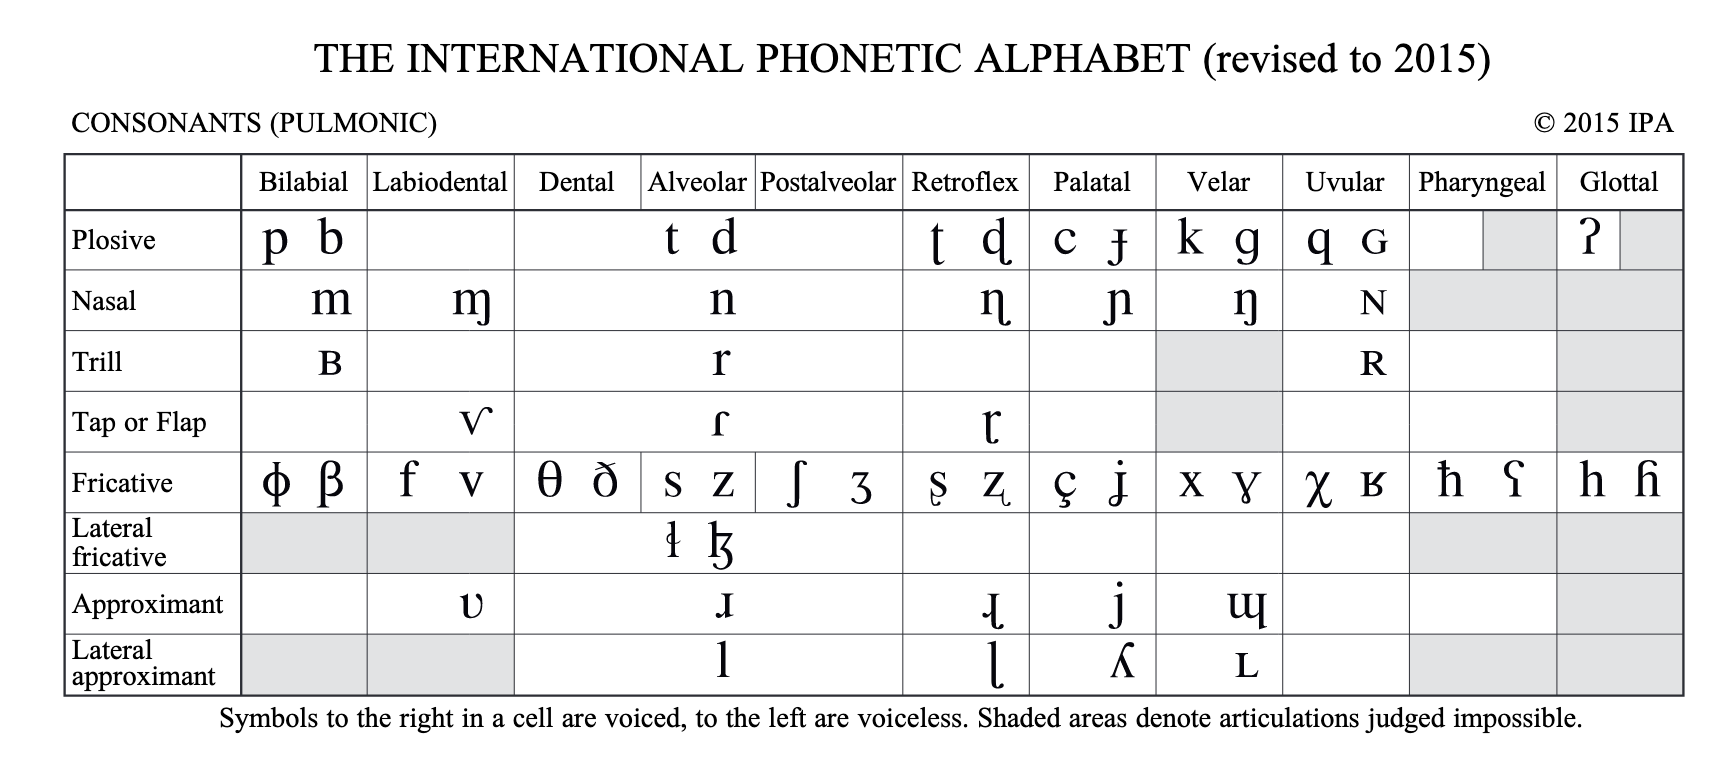
\includegraphics[width=\columnwidth]{second-midterm-2025/IPATABLE.png}\vspace{-1cm}
\end{center}

\end{enumerate}

\newpage
\Question{Speech Recognition: Fundamentals}{15}
\begin{enumerate}
\item The Source-Channel Model of Speech Recognition\hfill{\em (10 points)}
\begin{eqnarray}
\widehat{\mathbf{W}} &=& \arg\max_{\mathbf{W}}P(\mathbf{W}|\mathbf{A})\\
&=& \arg\max_{\mathbf{W}}\frac{P(\mathbf{A}|\mathbf{W})P(\mathbf{W})}{P(\mathbf{A})}\\
&=& \arg\max_{\mathbf{W}}P(\mathbf{A}|\mathbf{W})P(\mathbf{W})\\
&\approx& \arg\max_{\mathbf{W}}P_{\mathcal{A}}(\mathbf{A}|\mathbf{W})P_{\mathcal{L}}(\mathbf{W})
\end{eqnarray}
Explain, in one sentence each, why (2) is equal to (1), and why (3) is equal to (2).
\solution{
\begin{itemize}
\item (2) equals (1) by Bayes’ rule
\item argmax over W is insensitive to marginalization. [(3) = (2)] Since \(P(\mathbf{A})\) does not depend on \(\mathbf{W}\), it is constant under \(\arg\max_{\mathbf{W}}\) and can be dropped.
\end{itemize}}{}
Explain, in one sentence each, what the models $P_{\mathcal{A}}({\mathbf{A}|\mathbf{W})}$ and $P_{\mathcal{L}}(\mathbf{W})$ represent and what data is needed to train them.
\solution{
\begin {itemize}
\item Acoustic model, trained using large quantities of transcribed speech;
\item language model, trained using a large text corpus.\end{itemize}}{\vspace{1.5in}}
\item What factors make the automatic transcription of a group meeting more challenging than a news broadcast?\hfill{\em (5 points)}
 
\solution{Group meetings are usually spontaneous and conversational between everyday people, recorded in normal rooms, and recorded using distant microphones, while news broadcasts feature professional speakers who often read from a teleprompter in quite studios while wearing a lapel or head-mounted microphone.  Finally, text documents are available in the same style, and sometimes even on the same topics, entities and events being talked about in a news broadcast. \\
Spontaneous speech has co-articulation, mispronunciations and disfluencies; reverberation and background noises degrade audio recorded with distant microphones; multi-speaker conversations often overlapped speech; speech transcripts are not as abundant as news text for language modeling.}{\vspace{2cm}}
\end{enumerate}


\newpage
\Question{Speech Recognition: Neural Models}{20}
\vskip .25in
\begin{enumerate}
\item Draw a block diagram of an ASR system with an Encoder-Decoder-with-Attention architecture.  Label the audio $\mathbf{A}=a_1,a_2,\ldots,a_T$, the transcript $\mathbf{W}=w_1,w_2,\ldots,w_N$.  Draw arrows to illustrate (i) the system modules they go into or come out of, and (ii) the computational dependencies between the system modules.\hfill{\em (7 points)}

\solution{
\begin{figure}[h]
    \centering
    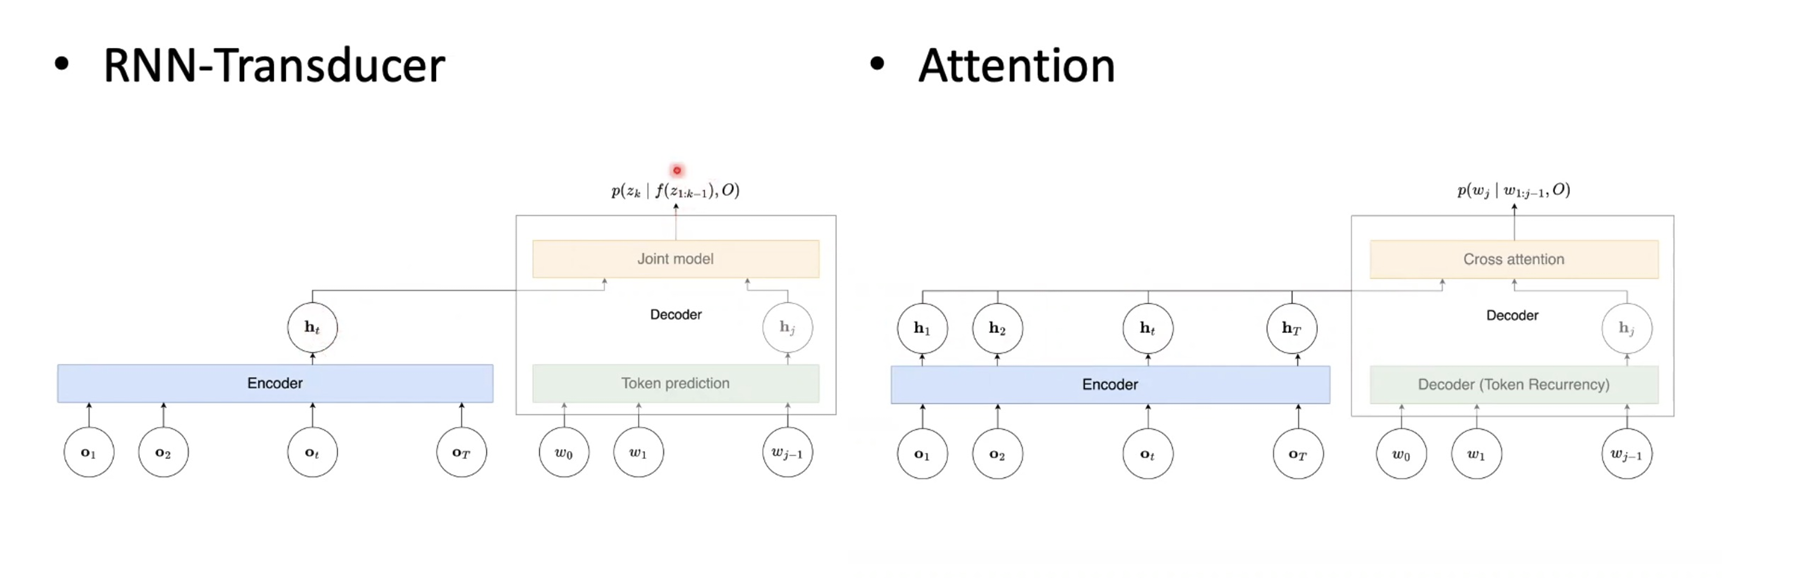
\includegraphics[width=0.7\linewidth]{second-midterm-2025/encoder-decoder.png}
    \caption{encoder-decoder ASR}
    %\label{fig:enter-label}
\end{figure}
Identify encoder, self- and cross-attention, and decoder blocks.  Decoder has both masked self-attention to its left and (masked or regular) cross-attention to the encoder outputs.}{\vspace{3.25in}}
\item Draw a block diagram of an ASR system with a Recurrent Neural Network Transducer architecture. Let $\mathbf{A}=a_1,a_2,\ldots,a_T$ and $\mathbf{W}=w_1,w_2,\ldots,w_N$ as above.  Draw arrows to illustrate (i) the system modules they go into or come out of, and (ii) the computational dependencies between the system modules.\hfill{\em (7 points)}

\solution{
\begin{figure}[h]
    \centering
    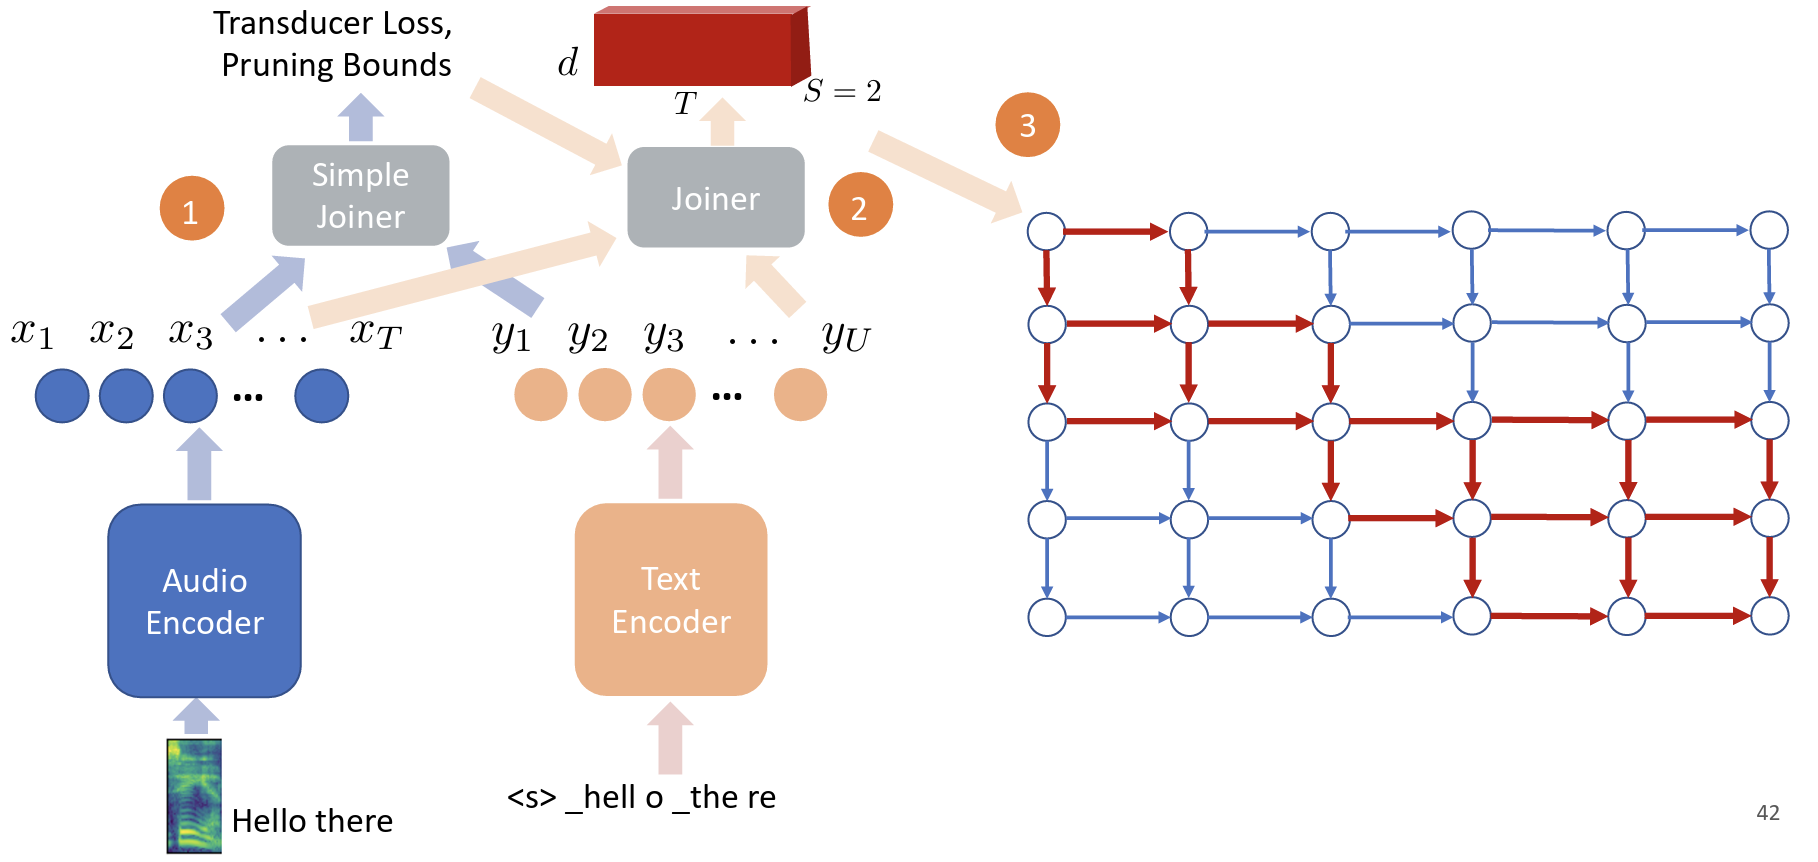
\includegraphics[width=0.7\linewidth]{second-midterm-2025/rnnt.png}
    \caption{RNNT for ASR}
    %\label{fig:enter-label}
\end{figure}\\
Identify the encoder, predictor and joiner blocks.  Indicate (somehow) that the joiner advances through the encoder output in a time-synchronous manner, but the predictor output advances in a symbol-synchronous manner.  E.g. show that to produce an output token $w_k$ at time frame $t$, the joiner joins the encoder frame $t$ with the predictor output based on $w_1,w_2,\ldots,w_{k-1}$.}{\vspace{3.25in}}
\item Which of the two architectures above requires a time-synchronous versus a label-synchronous decoder?  Which architecture is typically preferred for real-time/streaming applications? Which one seems a more natural fit for incorporating an external language model (or LLM)?\hfill{\em (6 points)}
\solution{EDA is symbol synchronous, RNN-T is time-synchronous.  RNN-T is preferred for real-time/streaming applications and is also ``easier'' for augmenting with an external LM.}{\vspace{3cm}}
\end{enumerate}

\newpage
\Question{Self-Supervised Learning for Speech}{15}
\begin{enumerate}
\item Draw a block-diagram to illustrate the architecture of a HuBERT model.\hfill{\em (3 points)}
\solution{\begin{figure}[h]
    \centering
    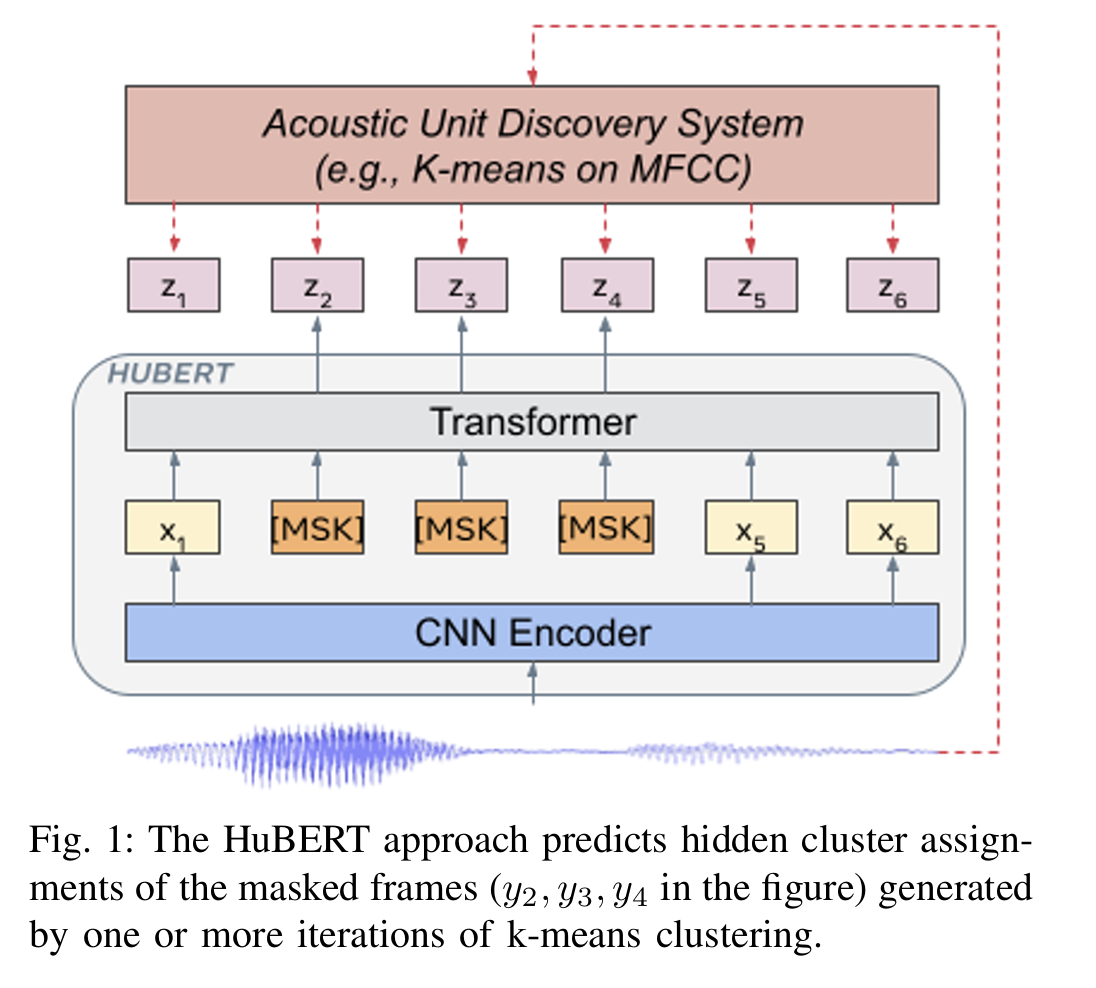
\includegraphics[width=0.5\linewidth]{second-midterm-2025/HuBERT.png}
    \caption{HuBERT}
    %\label{fig:enter-label}
\end{figure}.}{\vspace{2.5in}}
\item[] What training objective is used to train a HuBERT model?\hfill{(\em{2 points})}

\solution{BERT-like training with a masked language model objective}{\vspace{1in}}
\item[] How are VQ labels generated to train a HuBERT model?\hfill{(\em{2 points})}

\solution{Quantized MFCCs in the first iteration, quantized hidden layer in the second}{\vspace{1in}}
\item Draw a block-diagram to illustrate the architecture of wav2vec 2.0\hfill{\em (4 points)}
\solution{\begin{figure}[h]
    \centering
    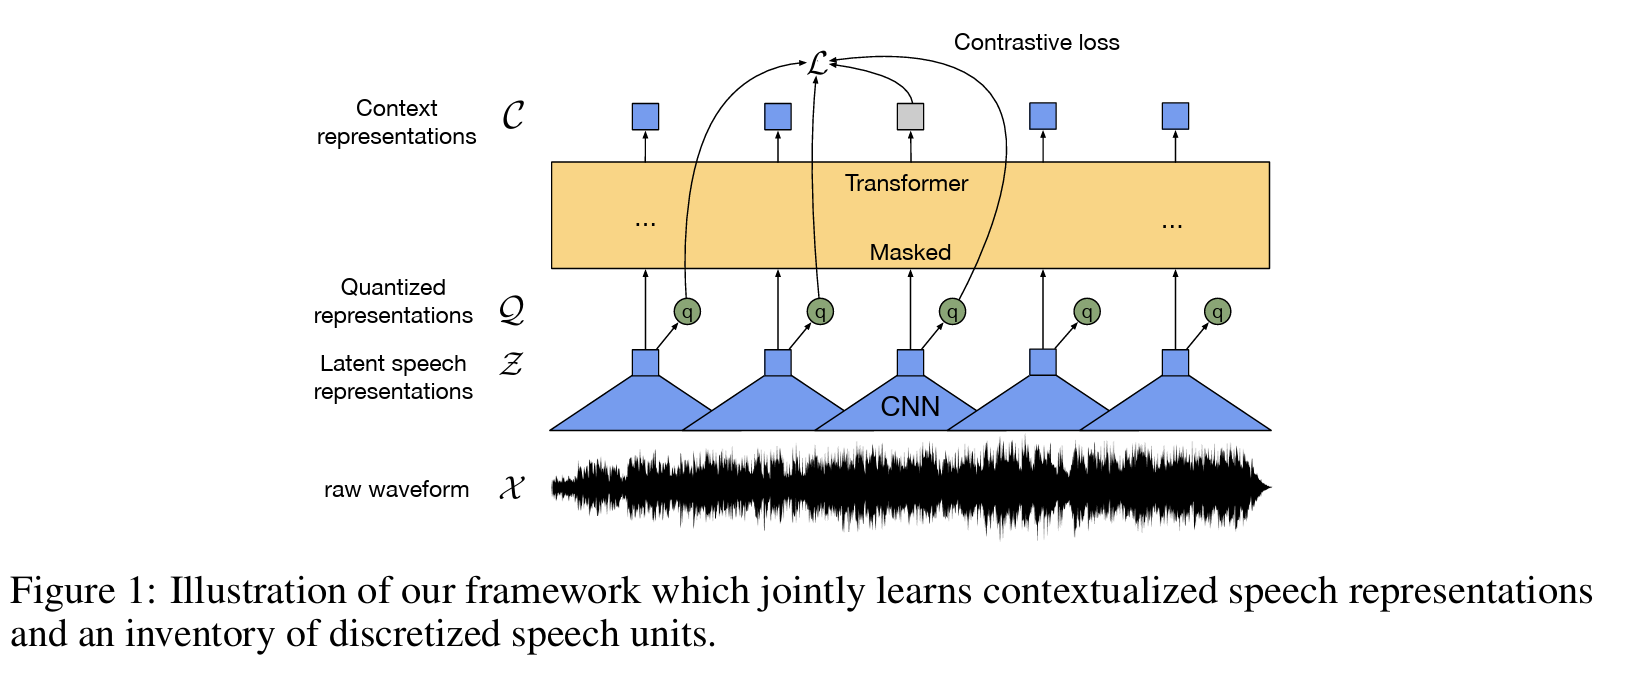
\includegraphics[width=0.7\linewidth]{second-midterm-2025/wav2vec.png}
    \caption{wav2vec}
    %\label{fig:enter-label}
\end{figure}.}{\vspace{2.5in}}
\item[] What training objective is used to train wav2vec 2.0?\hfill{(\em{2 points})}

\solution{Noise contrastive estimation, plus diversity/entropy of codebook use}{\vspace{1in}}
\item[] How are VQ centroids generated to train wav2vec 2.0?\hfill{(\em{2 points})}

\solution{The VQ centroids (aka codebook) are learnt iteratively as part of the training.}{\vspace{1in}}
\end{enumerate}


\newpage
\Question{Speaker Recognition}{20}
\vskip .25in

\begin{enumerate}
\item Draw the scheme of a generic speaker embedding network and explain the roles of the different parts of the network. Name different architecture choices for each one of the parts.   \hfill (8 points)\\
\solution{
\begin{figure}[h]
    \centering
    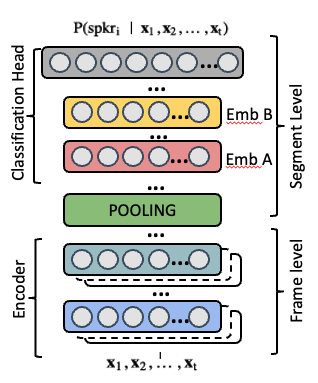
\includegraphics[width=0.5\linewidth]{second-midterm-2025/xvector.png}
    \caption{speaker embedding network (2 points)}
    %\label{fig:enter-label}
\end{figure}
X-Vector network has three parts:
\begin{itemize}
    \item Encoder: Gets log-Mel spectrogram features as input and produces speaker discriminant frame-level hidden representations as output. Different architectures in the literature include time-delay neural networks, 2d convolutional residual networks, and ecapa-tdnn networks (2 points).
    \item Pooling: Summarizes the frame-level hidden representations into a single vector per audio. Some methods are global mean pooling, global statistics pooling (mean+standard deviation), attentive statistics pooling, multi-head attention and channel-wise attentive statistics pooling (2 points).
    \item Classification Head: Predicts posterior probabilities for the training speakers given the pooling vector. At inference time, we extract the speaker embedding from a middle layer of the classification head (2 points).
\end{itemize}
}{\vspace{5cm}}
\newpage 

\item Define the probability of false alarm and probability of false rejection and how to calculate them \hfill (4 points) \\
\solution{\begin{itemize}
\item $P_\text{fa}$: Is the probability for an impostor to be classified as a true target speaker. This is calculated by setting a decision threshold on the speaker verification scores, counting the number of times an impostor is accepted and dividing by the total number of impostor trials.
\item $P_\text{fr}$: Is the probability for true target speaker to be classified as an impostor. This is calculated by setting a decision threshold on the speaker verification scores, counting the number of times an true target is rejected and dividing by the total number of target trials.
\end{itemize}
}{\vspace{5cm}}

\item Explain how to plot the Detection Error Trade-off curve and how to calculate the EER \hfill (4 points) \\
\solution{\begin{itemize}
\item DET curve plots the prob. of false alarm in the x-axis versus the prob. of false rejection or miss in the y-axis. To calculate it, we need to move the detection threshold from the minimum to the maximum score in our test scores. For each threshold value, we calculate the prob. of miss and prob. of false alarm. This gives us a point of the curve. The pairs of $(P_\text{fa}, P_\text{fr})$ for all thresholds give us the full curve
\item The EER is the point in the curve where the prob of false alarm is equal to prob. of rejection EER=$P_\text{fa}=P_\text{fr}$.
\end{itemize}
}{\vspace{5cm}}

\item Suppose you have an SV system that produces well-calibrated log-likelihood ratios, and you want to use it on an application where the prior probability of observing a target trial (true user) is $P_T$. Derive the formula for the decision threshold that we need to apply to the log-likelihood ratio. \hfill (4 points)\\
\solution{\begin{itemize}
\item To accept a target trial, the posterior probability for target trial has to be $P(T|x_e, x_t)\le 0.5$.
\item Write the posterior as a function of the LLR using Bayes Theorem:\\
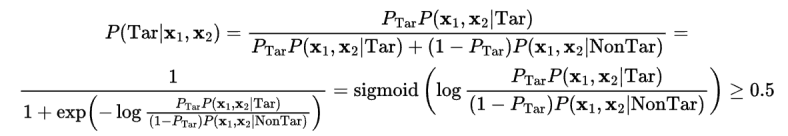
\includegraphics[width=0.9\linewidth]{second-midterm-2025/ptar.png}
\item Isolate the LLR from the eq. above:
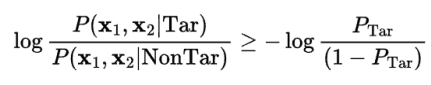
\includegraphics[width=0.5\linewidth]{second-midterm-2025/threshold.png}
\end{itemize}
}{\vspace{2cm}}
\end{enumerate}

\newpage
\Question{Enhancement and Diarization}{15}
\begin{enumerate}
\item Reverberation is a property of rooms, and its effect (given an acoustic source location and an observation point) is captured by the Room Impulse Response (RIR).

\begin{enumerate}

\item[a.] What do the direct path, early reflections, and late tail components of the RIR capture?
\hfill{\em (3 points)}
\solution{
\begin{itemize}
    \item (1pt) The direct path captures the delay and attenuation due to propagation from source to mic
    \item (1pt) The early reflections capture the first few reflections off walls and surfaces
    \item (1pt) The late tail is when the audio has reflected many times and resembles random noise
\end{itemize}
}{\vspace{5cm}}

\item[b.] What is the effect of reverberation on the spectrogram and why does it make enhancement difficult?
\hfill{\em (2 points)}
\solution{
\begin{itemize}
    \item (1pt) Reverberation smears the spectrogram
    \item (1pt) It is difficult to discriminate between the speech and the reverberation
\end{itemize}
}{\vspace{5cm}}

\item[c.] What is the most common approach to dereverberation and what is the idea behind the method?
\hfill{\em (2 points)}
\solution{
\begin{itemize}
    \item (1pt) Weighted Prediction Error (WPE)
    \item (1pt) Reverberation is essentially a linear function of the direct path observations and an inverse filter can be estimated
\end{itemize}
}{\vspace{5cm}}

\end{enumerate}
\newpage

\item What are the two primary diarization metrics, and give one example for each where that metric would be better for that conversational dynamic/application
\hfill{\em (4 points)}
\solution{
\begin{itemize}
    \item The metrics are (1pt) Diarization Error Rate (DER) and (1pt) Jaccard Error Rate (JER)
    \item (2pt) The basic difference is that DER is normalized by the amount of speech and JER is averaged over people in the recording. So, the examples should capture that JER is better if you care about individuals regardless of how much they speak, and DER is better if you care about overall performance.
\end{itemize}
}{\vspace{8cm}}

\item What is the foundational neural diarization system, and what was the ``trick'' required to make it work? Give one upside and one downside of this approach compared to conventional pipeline systems.
\hfill{\em (4 points)}
\solution{
\begin{itemize}
    \item (1pt) The model is End-to-End Neural Diarization (EEND)
    \item (1pt) Solving the problem that output order does not matter (i.e. the ``permutation problem''). This was done using approaches from speech separation (Permutation Invariant Training (PIT) and Deep Clustering)
    \item (1pt) Upsides include: joint optimization of the entire task and naturally handling overlapped speech
    \item (1pt) Downsides include: requiring lots of conversational data and having problematic model memory requirements for long-term recordings
\end{itemize}
}{\vspace{2cm}}

\end{enumerate}

\newpage

\textbf{\Large Extra Space}
\end{document}
